\documentclass[13pt,a4paper]{article}
\usepackage[spanish,es-nodecimaldot]{babel}	% Utilizar español
\usepackage[utf8]{inputenc}					% Caracteres UTF-8
\usepackage{graphicx}						% Imagenes
\usepackage[hidelinks]{hyperref}			% Poner enlaces sin marcarlos en rojo
\usepackage{fancyhdr}						% Modificar encabezados y pies de pagina
\usepackage{float}							% Insertar figuras
\usepackage[textwidth=390pt]{geometry}		% Anchura de la pagina
\usepackage[nottoc]{tocbibind}				% Referencias (no incluir num pagina indice en Indice)
\usepackage{enumitem}						% Permitir enumerate con distintos simbolos
\usepackage[T1]{fontenc}					% Usar textsc en sections
\usepackage{amsmath}						% Símbolos matemáticos
\usepackage[ruled,vlined]{algorithm2e}      % Pseudocódigo
\usepackage{xcolor}
\usepackage{listings}
% Para que acepten tíldes los listing
\lstset{     
     literate=%
         {á}{{\'a}}1
         {é}{{\'e}}1
         {í}{{\'i}}1
         {ó}{{\'o}}1
         {ú}{{\'u}}1
         {Á}{{\'A}}1
         {É}{{\'E}}1
         {Í}{{\'I}}1
         {Ó}{{\'O}}1 
         {Ú}{{\'U}}1
         {ñ}{{\~n}}1 
         {Ñ}{{\~N}}1 
         {¿}{{?``}}1 
         {¡}{{!``}}1
}
\usepackage{dsfont}

% ==============================================================================

\usepackage{caption, subcaption}
\usepackage[section]{placeins}
\makeatletter
\def\fps@figure{H}
\makeatother

\usepackage{booktabs}
\usepackage{longtable}
\usepackage{array}
\usepackage{multirow}
\usepackage{wrapfig}
\usepackage{colortbl}
\usepackage{pdflscape}
\usepackage{tabu}
\usepackage{threeparttable}
\usepackage{threeparttablex}
\usepackage[normalem]{ulem}
\usepackage{makecell}
\usepackage{xcolor}
\usepackage[bottom]{footmisc}

\makeatletter
\newcommand*{\centerfloat}{%
  \parindent \z@
  \leftskip \z@ \@plus 1fil \@minus \textwidth
  \rightskip\leftskip
  \parfillskip \z@skip}
\makeatother

% ==============================================================================
% ==============================================================================

% Comando para poner el nombre de la asignatura
\newcommand{\asignatura}{Aplicaciones de Ciencia de Datos y Tecnologías Inteligentes}
\newcommand{\autor}{Ignacio Vellido Expósito}
\newcommand{\email}{ignaciove@correo.ugr.es \\ 79056166Z}
\newcommand{\titulo}{Técnicas de Soft Computing}
\newcommand{\subtitulo}{Manejo de rutas y localización de aseos}

% Configuracion de encabezados y pies de pagina
\pagestyle{fancy}
\lhead{\autor{}}
\rhead{\asignatura{}}
\lfoot{Máster Ciencia de Datos e Ingeniería de Computadores}
\cfoot{}
\rfoot{\thepage}
\renewcommand{\headrulewidth}{0.4pt}		% Linea cabeza de pagina
\renewcommand{\footrulewidth}{0.4pt}		% Linea pie de pagina

% ==============================================================================
% ==============================================================================

\begin{document}
    \pagenumbering{gobble}
    % ==============================================================================
% Pagina de titulo
\begin{titlepage}
    \begin{minipage}{\textwidth}
        \centering

        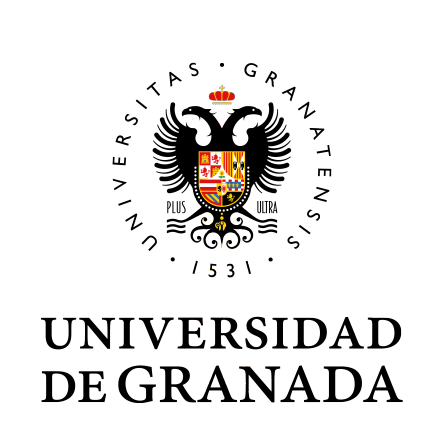
\includegraphics[scale=0.5]{img/ugr.png}\\

        \textsc{\Large \asignatura{}\\[0.2cm]}
        \textsc{MÁSTER CIENCIA DE DATOS E INGENIERÍA DE COMPUTADORES}\\[1cm]

        \noindent\rule[-1ex]{\textwidth}{1pt}\\[1.5ex]
        \textsc{{\Huge \titulo\\[0.5ex]}}
        \textsc{{\Large \subtitulo\\}}
        \noindent\rule[-1ex]{\textwidth}{2pt}\\[2.5ex]

        \end{minipage}

        \vspace{0.3cm}

        \begin{minipage}{\textwidth}

        \centering

        \textbf{Autor}\\ {\autor{} \\ ignaciove@correo.ugr.es}\\[1.5ex]
        \vspace{0.4cm}

        
\includegraphics[scale=0.3]{img/etsiit.jpeg}
        
\includegraphics[scale=0.6]{img/master.png}

        \vspace{0.7cm}
        \textsc{Escuela Técnica Superior de Ingenierías Informática y de Telecomunicación}\\
        \vspace{1cm}
        \textsc{Curso 2020-2021}
    \end{minipage}
\end{titlepage}
% ==============================================================================
    
    \pagenumbering{arabic}
    \tableofcontents
    \thispagestyle{empty}				% No usar estilo en la pagina de indice

    \newpage

    % ==============================================================================

    % \section{Resultados globales}

Orden usado en las técnicas:
Under/Oversampling > NoiseFiltering > Instance Selection

\begin{figure}[ht]
    \centerfloat
    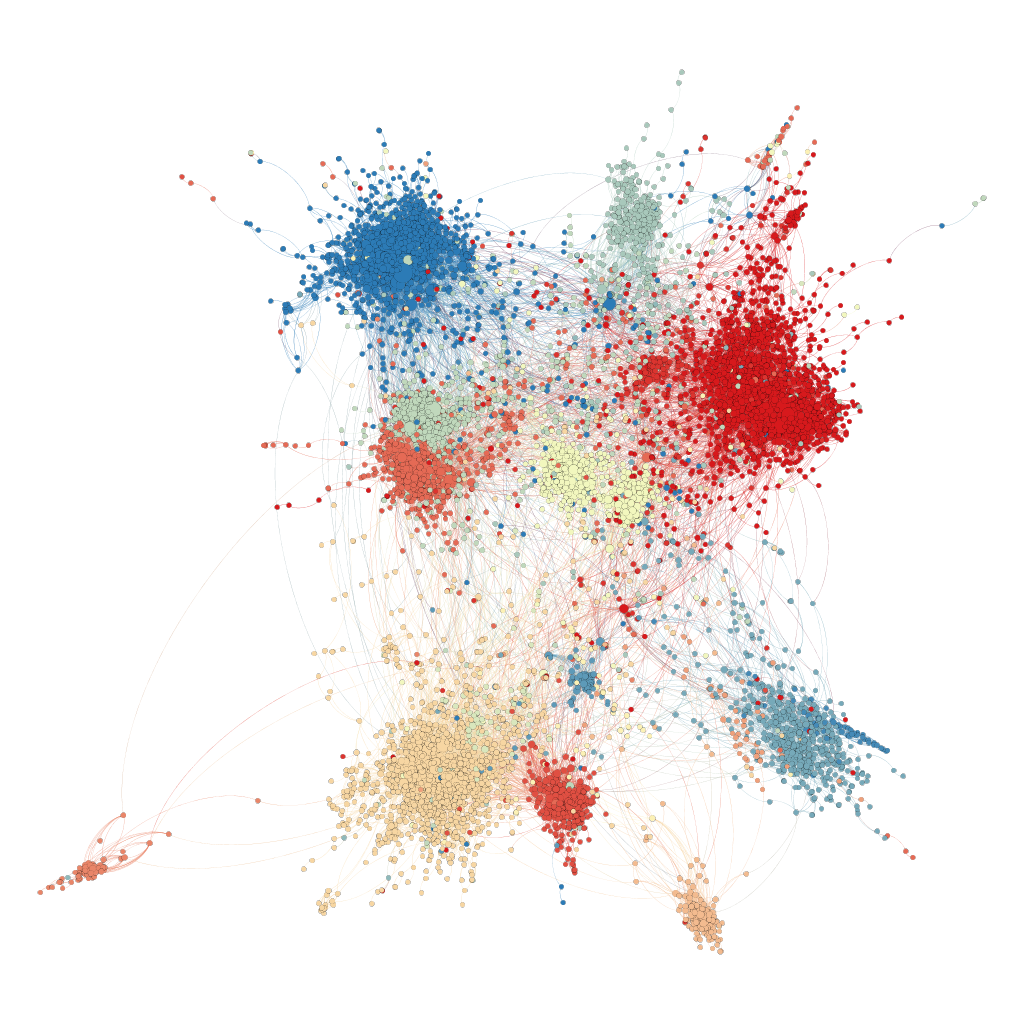
\includegraphics[width=1.097\textwidth]{img/resultados/grado-targets.png}
    \caption{Topología de la red. El color indica el país de cada usuario.}
\end{figure}

\begin{figure}[t]
    \centering
    \resizebox{0.78\columnwidth}{!}{%
    \begin{tabular}{| l | r |} 
        \hline
        \textbf{Medida} & \textbf{Valor} \\
        \Xhline{2\arrayrulewidth}
        Número de nodos \textbf{N} & 7,624 \\
        \hline
        Número de enlaces \textbf{L}	& 27,806 \\
        \hline
        Número máximo de enlaces \textbf{$L_{max}$} & 58117752 \\
        \hline
        Densidad del grafo \textbf{$L/L_{max}$} & 0.001 \\
        \Xhline{2\arrayrulewidth}
        Grado medio \textbf{<k>} & 7.294 \\
        \hline
        Diámetro \textbf{$d_{max}$} & 15 \\
        \hline
        Distancia media \textbf{d} & 5.232237269 \\
        \hline
        Coeficiente medio de clustering \textbf{<C>} & 0.285 \\
        \Xhline{2\arrayrulewidth}
        Número de componentes conexas & 1 \\
        \hline
        Número de nodos componente gigante (y \%) & 7,624 (100) \\
        \hline
        Número de aristas componente gigante (y \%) & 27,806 (100) \\
        \hline
    \end{tabular}
    }
    \caption{Medidas globales de la red.}
\end{figure} \newpage

% ¿A quíen no le ha dado alguna vez un apretón en la calle? Bueno, no hay forma de evitar que eso ocurra, pero podemos ayudar a hacer el problema más ameno

% ---------------------------

\section{Introducción}

Público objetivo: Personas con problemas intestinales, turistas, gente que trabaja en la calle (taxistas)
Probablemente mejor aceptado por gente del rango 25-40, al resto les puede dar vergüenza.

Es necesaria la colaboración extrema y constante de los usuarios para crear la comunidad. Los principios de la app serán difíciles

% Vaguedad en los datos
% Propuesta, solo documentación

\section{Descripción del sistema}

% Gráfico global

\subsection{Subsistema de entrada}

- Urgencia: El usuario podrá elegir entre diferentes niveles de urgencia ("inmediato", "pronto", "más adelante") que se tendrán en cuenta a la hora de calcular la distancia y los niveles de calidad aceptados.
- Ubicación: Mediante el geo-localizador del móvil, o incluso la posibilidad de introducirlo a mano si se pretende estimar de antemano.
- (Opcional) Criterios de higiene: Se usaran 3 etiquetas lingüísticas ("impecable", "limpio", "sucio") que devolverá el sistema
- (Opcional) Género: Para filtrar los resultados de las reviews.

También, adicionalmente
El usuario podría limitar el tipo de sitios en los que acepta a ir, pues por ejemplo sería de mal gusto entrar una cafetería sin consumir nada.

Entre posibles tipos de locales: Restaurantes y cafeterías, universidades, estaciones de tren y bus, edificios públicos, centros comerciales, baños públicos, incluso su propia vivienda (para darle mayor prioridad)

\subsection{Subsistema central}

Primeramente será necesario cuantificar los niveles cualitativos introducidos por el usuario.

A partir de la ubicación, la urgencia y los criterios de higiene se estima un radio máximo de posibles baños (fórmula)

Seguidamente, se extrae la información de los baños desde la base de datos (valores de higiene, distancia, ocupación) y se aplica un algoritmo de optimización siguiendo el esquema:

Maximizar la higiene, disminuir la distancia, disminuir la probabilidad de ocupación
tal que:
higiene <= criterio mínimo de higiene (restricción flexible)
distancia <= (tiempo estimado en llegar)

Se podría asociar una puntuación a cada baño en base a la siguiente forma:

Estos baños se ordenan en base a su puntuación y pasa al sistema 

\subsection{Subsistema de salida}

Subsistema de Salida, que brindará la información geográfica de la ruta adaptada. Usará etiquetas lingüísticas para brindar las informaciones y recomendaciones de las rutas de forma cualitativa.
La parte inteligente del sistema respecto a la gestión de adaptación de la ruta es la Base de Reglas Difusas, que será descrita a continuación, y en la que se presentará el diseño del controlador difuso que “deforma” la información de la ruta, describiendo las variables de estado, sus respectivas funciones de pertenencia, y la base de reglas correspondiente

Transformará las etiquetas lingüísticas en representaciones gráficas para un mejor aspecto visual de la aplicación.

Si el resultado es exitoso la aplicación devuelve, de forma ordenada al score puntuado, 3 posibles localizaciones con la siguiente información:

\begin{itemize}
  \item Nombre.
  \item Información geográfica de la ruta más corta desde la ubicación del usuario hasta el lugar, mostrando la distancia y el tiempo de llegada aproximado.
  \item Probabilidad de estar ocupado.
  \item Nivel de higiene estimado.
\end{itemize}
% Probabilidad de estar ocupado: En base a la cantidad de gente en la zona. Una base de datos adicional (propia o con información introducida por los usuario) podría aportar conocimiento adicional sobre el número de baños, la ubicación (ej: si se encuentra en el bajo de un apartamento es de esperar que aparente haber más gente de la que hay). etc.
- Nivel de higiene: A partir de las reviews de los usuarios. También se podría hacer un estudio de ciencia de datos recogiendo datos de la ubicación, número de personas, fecha y hora\dots, con el objetivo de predecir el nivel de higiene en ese momento.

Información de si están rotos

Si por el contrario no hubiera éxito en el cálculo de los locales, la aplicación ofrecería al usuario recalcular las rutas relajando los posibles criterios (o también, si el sistema base es capaz de responde rápidamente, calcularlos en la primera llamada y ofrecerlos indicando las restricciones).

% Inicialmente, el sistema solicita al usuario que indique cuánto está dispuesto a desplazarse
% dada su ubicación actual. La base lógica difusa se encarga de convertir esta información
% cualitativa a cuantitativa mediante un proceso de “defuzzicación”.Así, ya esta información se
% utiliza a modo de filtro la API de TripAdvisor [5] para obtener los mejores locales de tapas en
% ese radio.

    % ==============================================================================

    \setlength{\parskip}{1em}
    \newpage
    % \nocite{*}
    % \bibliography{bibliografia}
  	% \bibliographystyle{plain}
\end{document}